%%
%% This is file `sample-manuscript.tex',
%% generated with the docstrip utility.
%%
%% The original source files were:
%%
%% samples.dtx  (with options: `manuscript')
%% 
%% IMPORTANT NOTICE:
%% 
%% For the copyright see the source file.
%% 
%% Any modified versions of this file must be renamed
%% with new filenames distinct from sample-manuscript.tex.
%% 
%% For distribution of the original source see the terms
%% for copying and modification in the file samples.dtx.
%% 
%% This generated file may be distributed as long as the
%% original source files, as listed above, are part of the
%% same distribution. (The sources need not necessarily be
%% in the same archive or directory.)
%%
%% The first command in your LaTeX source must be the \documentclass command.
%%%% Small single column format, used for CIE, CSUR, DTRAP, JACM, JDIQ, JEA, JERIC, JETC, PACMCGIT, TAAS, TACCESS, TACO, TALG, TALLIP (formerly TALIP), TCPS, TDSCI, TEAC, TECS, TELO, THRI, TIIS, TIOT, TISSEC, TIST, TKDD, TMIS, TOCE, TOCHI, TOCL, TOCS, TOCT, TODAES, TODS, TOIS, TOIT, TOMACS, TOMM (formerly TOMCCAP), TOMPECS, TOMS, TOPC, TOPLAS, TOPS, TOS, TOSEM, TOSN, TQC, TRETS, TSAS, TSC, TSLP, TWEB.
% \documentclass[acmsmall]{acmart}

%%%% Large single column format, used for IMWUT, JOCCH, PACMPL, POMACS, TAP, PACMHCI
% \documentclass[acmlarge,screen]{acmart}

%%%% Large double column format, used for TOG
% \documentclass[acmtog, authorversion]{acmart}

%%%% Generic manuscript mode, required for submission
%%%% and peer review
%\documentclass[manuscript,screen]{acmart}
\documentclass[sigchi, review]{acmart}

%%
%% \BibTeX command to typeset BibTeX logo in the docs
\AtBeginDocument{%
  \providecommand\BibTeX{{%
    \normalfont B\kern-0.5em{\scshape i\kern-0.25em b}\kern-0.8em\TeX}}}

%% Rights management information.  This information is sent to you
%% when you complete the rights form.  These commands have SAMPLE
%% values in them; it is your responsibility as an author to replace
%% the commands and values with those provided to you when you
%% complete the rights form.
%\setcopyright{acmcopyright}
\copyrightyear{2020}
%\acmYear{2020}
%\acmDOI{10.1145/1122445.1122456}

%% These commands are for a PROCEEDINGS abstract or paper.
%\acmConference[Woodstock '18]{Woodstock '18: ACM Symposium on Neural
 % Gaze Detection}{June 03--05, 2018}{Woodstock, NY}
%\acmBooktitle{Woodstock '18: ACM Symposium on Neural Gaze Detection,
 % June 03--05, 2018, Woodstock, NY}
%\acmPrice{15.00}
%\acmISBN{978-1-4503-XXXX-X/18/06}
\usepackage{booktabs}
\usepackage{bbding}
\usepackage{pifont}
\usepackage{wasysym}
\usepackage{amssymb}
%%
%% end of the preamble, start of the body of the document source.
\begin{document}

%%
%% The "title" command has an optional parameter,
%% allowing the author to define a "short title" to be used in page headers.
\title{A Survey of Augmented Piano Prototypes}

%%
%% The "author" command and its associated commands are used to define
%% the authors and their affiliations.
%% Of note is the shared affiliation of the first two authors, and the
%% "authornote" and "authornotemark" commands
%% used to denote shared contribution to the research.
\author{Jordan Aiko Deja}

\orcid{1234-5678-9012}
\affiliation{%
  \institution{University of Primorska}
  \city{Koper}
  \country{Slovenia}
  \postcode{6000}}
\email{jordan.deja@famnit.upr.si}

\author{Matjaž Kljun}
\affiliation{%
  \institution{University of Primorska}
  \city{Koper}
  \country{Slovenia}
  \postcode{6000}}
\email{matjaz.kljun@famnit.upr.si}

\author{Klen Čopič Pucihar}
\affiliation{%
  \institution{University of Primorska}
 \city{Koper}
  \country{Slovenia}
  \postcode{6000}}
\email{klen.copic@famnit.upr.si}

%%
%% By default, the full list of authors will be used in the page
%% headers. Often, this list is too long, and will overlap
%% other information printed in the page headers. This command allows
%% the author to define a more concise list
%% of authors' names for this purpose.
\renewcommand{\shortauthors}{Deja, et al.}
%%
%% The abstract is a short summary of the work to be presented in the
%% article.
\begin{abstract}
\textbf{Abstract:} change this abstract in line with the prisma checklist jordan. Humans have been using and learning the piano for over 3 centuries. In the last 15 years, several Augmented Reality (AR) piano prototypes that support learning have been introduced. What are the different developments and contributions in terms of AR piano prototype development? Why are we still building these prototypes? What do these systems lack? In this paper, we present a systematic review of AR piano prototypes developed within the recent years. We review the different innovations they present and organise them into contribution categories. We will then discuss the impact of these contributions and recommend directions for future work towards designing better AR piano prototypes and conducting user studies.
\end{abstract}
%%
%% The code below is generated by the tool at http://dl.acm.org/ccs.cfm.
%% Please copy and paste the code instead of the example below.
%%
\begin{CCSXML}
<ccs2012>
   <concept>
       <concept_id>10003120.10003138.10011767</concept_id>
       <concept_desc>Human-centered computing~Empirical studies in ubiquitous and mobile computing</concept_desc>
       <concept_significance>500</concept_significance>
       </concept>
 </ccs2012>
\end{CCSXML}
\ccsdesc[500]{Human-centered computing~Empirical studies in ubiquitous and mobile computing}
%%
%% Keywords. The author(s) should pick words that accurately describe
%% the work being presented. Separate the keywords with commas.
\keywords{augmented reality, piano, meta-analysis, prototypes}
%%
%% This command processes the author and affiliation and title
%% information and builds the first part of the formatted document.
\maketitle

\section{Introduction}
In around the year 1700, the piano, an elegant yet complex to use musical instrument was invented. Since then, humans have been designing innovations improving the experiences of learning and playing the piano. Several technology interventions have been introduced to assist in these scenarios. As these contributions are presented, changes in the way humans use the piano and technology also take place. This is because of the affordances affecting users that go with these technologies. One of these innovations is through Augmented Reality (AR). The earliest known prototype designed with AR came in the late 90s in the form of a musical keyboard display with keyboard input method \cite{breitweiser1996musical}. This along with other AR prototypes rode the waves of the Information era, with the boom of the World Wide Web, the emergence of the millennium bug, higher resolution graphics, stronger processors and better tracking algorithms among many others. Since then, as several AR piano prototypes have been developed, key innovations have shifted focus as well jumping from one technology to other (e.g. overlaying graphics to optimization to teaching modes). As these innovations shift focus from one to the other, human experiences are also reshaped by these changes. 

\citet{dede1996evolution} contends that technological media (such as computers) provide affordances that play an important role in the use and teaching with technology. Therefore, it is important to study how learning a music instrument augmented with digital technology and how such innovations can be maximized to improve and sustain piano learning experiences. A study by \citet{tamim2011forty} shows us that the use of technology can help learners improve their over-all performance. We believe that the same approach can be made applicable in piano learning as well. This is why we think that several prototypes and technologies have been developed for the piano. 

This introduction is not yet done. I need to elaborate the second and third question in the abstract. 

Several technologies have enabled the creation of hardware, learning modes and interactive spaces. Over the last 20 years, we have observed progress in hardware computing power, tracking of elements in real-time (such has hand, object tracking) and in authoring AR tools, plug-ins and applications. These technologies are already seen and applied in several settings such as in tourism \cite{kounavis2012enhancing}, learning \cite{santos2013augmented}, manufacturing \cite{thomas1992augmented}, pilot training \cite{macchiarella2004augmented} and many others. As a first goal, this paper aims to review the different trends and categories that have improved AR experiences with special emphasis to the piano. Even though there have been several AR piano prototypes in current literature, we believe that only a few are developed with focus on improving how piano novices learn (and towards having sustainable, meaningful learning experiences). The different novel contributions in piano AR have been measured to be effective based on several metrics such as registration speed, quality of graphics, and observed learner performance. These studies have been written with a distinct context in mind. As such, replicating these studies will depend on various factors such as: accessibility of required hardware, difficulty of recreating assets, available open-source libraries and willing participants for user studies. As a second goal, we intend to guide researchers on possible directions towards introducing novel contributions in AR piano prototypes. We shall do this by summarizing the state-of-the-art implementation and evaluation of included literature. Then, we enumerate recommendations for learning piano with AR and discuss relevant innovations and models that can support these recommendations. 

The paper is organized as follows: Section \ref{sec: bg}  discusses our definition of Augmented Reality (AR) piano prototypes and a background on the piano learning process. Section \ref{sec: method} describes our methods for qualitative analysis. Section \ref{sec: trends} discusses the results of our analysis of the trends in AR piano prototypes designed throughout the years. These include state-of-the-art contributions (in the design, engineering and content). We organise these strategies into categories such as hand tracking, visualisations, agents and tutors, and learning modes and discuss each of them in Section \ref{sec: strat}. Lastly, Section \ref{sec: discuss} concludes this paper with our recommendation for future AR piano prototypes. 

\section{Background}
\label{sec: bg}
% focus on piano and musical instruments 
%\subsection{Piano Learning}
How do people learn the piano? what are the different stages of learning the piano? what stages in piano learning have been augmented by technology? what are the existing gaps in this process? How much virtuality (in miligram's continuum) has been included in piano? 

%\subsection{Augmented Reality Piano Prototypes}
Augmented Reality
Augmented reality piano teaching systems
Design Factors affecting augmented reality piano teaching systems (hardware, software, content)

\section{Method}
\label{sec: method}
We did a literature review following the \textit{Preferred Reporting Items for Systematic Reviews and Meta-Analyses} technique, also known as \textbf{PRISMA} \cite{moher2009preferred}. The work of \citet{santos2013augmented} which has reviewed AR learning environments has applied PRISMA techniques as well. This guided us further on how to analyse and review AR prototypes for this specific context. The approach included a  qualitative-analysis phase that aims to review these innovations in a specific context. The methodology for this systematic review is as follows: 

\subsection{Search for Prototypes}
\label{subsec: search}
We did a literature search between March to August 2020 in several digital libraries such as Google Scholar, ACM Digital Library and IEEE Xplore Digital Library. The search strings used where:
\begin{enumerate}
    \item "augmented reality piano"
    \item "AR piano"
    \item "augmented reality keyboard"
    \item "AR keyboard"
\end{enumerate}
The search included journal articles, conference proceedings and other articles that are written in English. Some articles were not written in English but had available translations. These were included as well. A total of 316 articles were found from this initial search from these online libraries. 
\subsection{Inclusion Criteria}
\label{subsec: criteria}
The focus of this survey is on AR piano prototypes. We needed to further filter these articles based on the following criteria:
\begin{enumerate}
    \item The paper discusses a prototype with the AR piano in focus.  
    \item The AR piano prototype is meant for playing, learning or teaching the piano.
    \item The prototype fits the description of augmented reality as seen in Section \ref{sec: bg}.
    %\item The full research paper is publicly accessible 
\end{enumerate}
These inclusion criteria were manually performed at the best judgment of the author. Following this criteria, we resulted to forty (40) articles. Moreover, not all these prototypes immediately qualify based on the definition of AR. Prototypes that make use of both 2D and 3D are considered. Prototypes that simulate the effect of AR even if they do not implement the tracking of an object were also included in this review. 

\subsection{Qualitative Analysis}
We performed a qualitative analysis of the different papers retrieved after performing the steps at subsection \ref{subsec: search}. We used the criteria defined in subsection \ref{subsec: criteria}. This gave us a clearer understanding of the prototypes in these articles. Note that these 40 articles do not represent 40 unique prototypes because a small fraction of these studies discussed advancements in the development of the same prototype.

\subsection{Data Gathering}
\label{subsec: gathering}
A form was drafted to facilitate the gathering of data from the 40 included articles. The form seeks to retrieve the following information: 
\begin{enumerate}
    \item publication details
    \item contributions
    \item use of AR
    \item citation count
    \item design and results of the user study
\end{enumerate}
The publication details include the title of the paper, year of publication, authors etc. The contributions of each paper were extracted and analyzed as well. The use of AR refers to the set of features that describe its AR component. This can refer to as head-mounted, agent-based, mobile, etc. The design and results of the user study refer to the description of applicable user studies and tests. Other features include sample size, method, questionnaire and tools used to conduct the user tests.

The review was designed to easily recognize common trends among the papers included in this study. Data and findings were sorted towards supporting any form of further data gathering. Note that the goal is not to correctly describe which prototype is an AR piano or not but to gather enough examples of prototypes that have effectively used AR as a technique in playing or learning the piano.  

\section{Trends in AR Piano Prototypes}

\begin{table*}[h]
\caption{Table of studies and a checklist of their features based on contribution categories as described in section \ref{sec: trends}.}
%\small
\begin{tabular}{llrrccccccl}
\hline \hline
\textbf{Paper} & \textbf{Author} & \textbf{Year} & \textbf{\#} & \textbf{KB} & \textbf{AT} & \textbf{PR} & \textbf{US} & \textbf{HT} & \textbf{LM} & \textbf{Others} \\ \hline
P1    & \citet{huang2011piano}              & 2011 & 50         & \ding{51} &           &           &           & \ding{51} &           & \\ \hline
P2    & \citet{nugraha2014pemanfaatan}      & 2014 & 38         & \ding{51} &           &           & \ding{51} &           &           & \\ \hline
P3    & \citet{barakonyi2005augmented}      & 2005 & 47         & \ding{51} & \ding{51} & \ding{51} &           &           & \ding{51} & \\ \hline
P4    & \citet{chow2013music}               & 2013 & 45         & \ding{51} &           & \ding{51} & \ding{51} &           & \ding{51} & \\ \hline
P5    & \citet{weing2013piano}              & 2013 & 29         &           &           & \ding{51} & \ding{51} & \ding{51} & \ding{51} & \textit{gamified viz}\\ \hline
P6    & \citet{hackl2017holokeys}           & 2017 & 7          & \ding{51} &           & \ding{51} &           &           &           & \\ \hline
P7    & \citet{chouvatut2013virtual}        & 2013 & 8          & \ding{51} &           & \ding{51} &           &           &           & \textit{supports PWD's}\\ \hline
P8    & \citet{fernandez2016piano}          & 2016 & 7          &           & \ding{51} & \ding{51} &           &           &           & \\ \hline
P9    & \citet{das2017music}                & 2017 & 5          & \ding{51} & \ding{51} & \ding{51} &           &           & \ding{51} & \textit{lesson builder} \\ \hline
P10   &  \citet{claudia2017yousician}       & 2017 & 0          &           &           & \ding{51} &           &           &           & \\ \hline
P11   & \citet{trujano2018arpiano}          & 2018 & 4          & \ding{51} &           & \ding{51} &           &           &           & \\ \hline
P12   & \citet{kerdvibulvech2017innovative} & 2017 & 4          & \ding{51} &           &           & \ding{51} & \ding{51} &           & \textit{users gesture on air}\\ \hline
P13   & \citet{oka2013marker}               & 2013 & 27         &           &           &           &           & \ding{51} &           & \textit{piano fingering}\\ \hline
P14   &  \citet{liang2016barehanded}        & 2016 & 20         & \ding{51} &           &           &           & \ding{51} &           & \\ \hline
P15   & \citet{schmalstieg2007experiences}  & 2007 & 268        &           &           & \ding{51} & \ding{51} &           &           & \\ \hline
P16   & \citet{correa2009computer}          & 2009 & 63         & \ding{51} &           & \ding{51} & \ding{51} &           &           & \textit{patients w/ cerebral palsy}\\ \hline
P17   & \citet{xiao2014andante}             & 2014 & 28         &           & \ding{51} & \ding{51} &           &           & \ding{51} & \\ \hline 
P18   & \citet{takegawa2012piano}           & 2012 & 26         &           &           & \ding{51} & \ding{51} &           & \ding{51} & \\ \hline 
P19   & \citet{xiao2010mirrorfugue}         & 2011 & 31         &           & \ding{51} & \ding{51} & \ding{51} &           &           & \textit{3 unique interfaces}\\ \hline
P20   & \citet{xiao2013mirrorfugue}         & 2013 & 17         &           & \ding{51} &           & \ding{51} &           &           & \\ \hline
P21   & \citet{li2018application}           & 2018 & 1          & \ding{51} &           &           & \ding{51} &           &           & \\ \hline 
%P22   & \citet{wei2015teaching}             & 2015 & 154        &                  &       &        &    &  & &             \\
P22   & \citet{zaqout2015augmented}         & 2015 & 1          & \ding{51} &           &           &           &           &           & \\ \hline 
%P24   & \citet{serafin2017considerations}   & 2017 & 25         &                  &       &         &   &  & &             \\
P23   & \citet{leonard2013virtual}          & 2013 & 9          & \ding{51} &           &           & \ding{51} &           &           & \\ \hline 
P24   & \citet{raymaekers2014game}          & 2014 & 14         &           &           & \ding{51} & \ding{51} &           & \ding{51} & \textit{shooting game}\\ \hline
P25   & \citet{rogers2014piano}             & 2017 & 42         &           &           & \ding{51} & \ding{51} &           & \ding{51} & \\ \hline
P26   & \citet{birhanu2017keynvision}       & 2017 & 2          &           &           & \ding{51} &           &           & \ding{51} & \\ \hline
P27   & \citet{sun2018mr}                   & 2018 & 3          & \ding{51} &           & \ding{51} & \ding{51} &           &           & \textit{one and two hand modes}\\ \hline
P28   & \citet{goodwin2013key}              & 2013 & 10         &           & \ding{51} & \ding{51} &           &           &           & \\ \hline
P29   & \citet{zeng2019funpianoar}          & 2019 & 2          &           &           &           &           &           &           & \textit{used ar markers}\\ \hline
P30   & \citet{de2014infrared}              & 2014 & 6          & \ding{51} &           &           &           & \ding{51} &           & \textit{magnetic glove}\\ \hline
P31   & \citet{molloy2019mixed}             & 2019 & 1          &           &           & \ding{51} & \ding{51} &           & \ding{51} & \textit{cognitive load, motivation}\\ \hline
%P34   &  \citet{zaqout2015augmented}        & 2015 & 1          &                  &       &          &  &      & &         \\
P32   & \citet{cai2019designa}               & 2019 & 1         &           &           & \ding{51} &           &           & \ding{51} & \textit{formal \& competition mode}\\ \hline
P33   & \citet{gerry2019adept}              & 2019 & 2          &           & \ding{51} & \ding{51} &           & \ding{51} &           & \textit{leap motion capture}\\ \hline 
P34   & \citet{zhang2010affordable}         & 2010 & 22         & \ding{51} &           &           &           &           &           & \\ \hline 
P35   &  \citet{pan2018pilot}               & 2018 & 2          & \ding{51} &           &           & \ding{51} &           &           & \textit{single \& pair modes}\\ \hline
P36   &  \citet{cai2019designb}              & 2019 & 0         &           &           & \ding{51} &           & \ding{51} &           & \textit{group piano}\\ \hline
%P40   &  \citet{poupyrev2001augmented}      & 2001 & 27         &                  &       &         &   &     & &          \\
P37   & \citet{sandnes2019enhanced}         & 2019 & 0          &           &           & \ding{51} &           &           &           & \\ \hline
P38   & \citet{kim2014ar}                   & 2014 & 11         & \ding{51} &           & \ding{51} & \ding{51} &           &           & \\ \hline
%P43   & \citet{zeng2019new}                 & 2019 & 0          &                  &       &        &    &    & &           \\
P39   &  \citet{xiao2011duet}               & 2011 & 7          &           &           & \ding{51} & \ding{51} &           & \ding{51} & \textit{practice modes}\\ \hline 
P40   & \citet{xu20195}                     & 2019 & 0          &           & \ding{51} & \ding{51} &           &           & \ding{51} & \textit{self reflection}\\ \hline 
%P46   & \citet{oku2019novel}                & 2019 & 2          &                  &       &         &   &     & &          \\
%P47   & \citet{birhanu2017interactive}      & 2017 & 0          &                  &       &         &   &      & &         \\
%P48   &  \citet{rahman2013hand}             & 2013 & 6          &                  &       &         &   &     & &          \\
%P49   & \citet{mostafizur2011application}   & 2011 & 5          &                  &       &         &   &       & &        \\ \hline
      &                                     &           & \textit{\={x}}=21 & 47\% & 22\% & 67\%    & 45\%      & 20\%      & 32\%      & \\ \hline \hline
\label{tab:overview}
\end{tabular}
\caption*{Legend: \textbf{\#}= number of citations; \textbf{KB}= AR keyboard; \textbf{AT}= AR agents and tutors; \textbf{PR}= piano roll and other visuals that simplify chords and notes; \textbf{US}= user study; \textbf{HT}= hand tracking; \textbf{LM}= learning modes.}
\end{table*}
\label{sec: trends}
Forty (40) articles discussing AR piano prototypes have been evaluated and reviewed in this paper. The data collected about these papers can be found in Table \ref{tab:overview}. Following the qualitative analysis and the data gathering that took place, we were able to come up with AR contribution categories for piano learning. These are (1) \textbf{KB}: an AR keyboard that is seen by or displayed to the users for them to \textit{"press"}; (2) \textbf{AT}: an AR agent or tutor that is designed to help the user play the piano; (3) \textbf{PR}: refers to the piano roll and other similar visualizations, guiding the users on what keys to  \textit{"press"} in the piano; (4) \textbf{US}: a form of evaluation with the users that intends to assess the usability of the AR piano prototype; (5) \textbf{HT}: use of hand tracking and similar technology to register, display and render graphics in space and (6) \textbf{LM}: refers to the set of interfaces and modes that the user can utilize in helping them learn the piano. These contributions were counted, marked and labeled as see in the table mentioned earlier. This provides the readers a simplified view of the contributions in AR piano prototypes. These data points were also sorted by year, by category type in order to visualize the trends that we have observed. The respective charts and graphs describing these trends can be found in Figure \ref{fig:doublechart}. From these figures, we show the rise and trends on AR prototypes within the last 2 decades. The most common contribution categories and how they are bundled together across the years can also be seen. 

The earliest prototype included in our systematic review was from the year 2005. However, while there have been patents and products filed as \textit{"augmented reality piano"} as early as the year 1998, these were not included in the review because of the inclusion criteria described in subsection \ref{subsec: criteria}. Also, details that allow the author to review these patents systematically were not easily-accessible.

Between the years 2005 to 2010, along with the rise of mobile technologies and better phone cameras (especially the iPhone \cite{querashi2012apple}), a handful of studies have attempted to develop AR piano prototypes. These studies featured an virtual keyboard and piano roll notation that users can operate with. We can say that these contribution categories have been the earliest attempts to innovate piano learning with AR. We believe that the primary focus during these years, was to make piano learning exciting by introducing a \textit{"virtual"} keyboard that can be viewed anywhere. As the typical piano instrument is heavy and bulky, having augmented keyboards was the obvious and portable approach to begin with. As humans were slowly shifting from personal computing to mobile computing, the trend in piano learning was also headed towards the same direction.

Between the years 2011 to 2015, an obvious rise of AR piano prototypes published can be seen. The most common contributions during this period was the piano roll visualization. As mobile devices and their cameras were getting more powerful during this period, we believe that the focus may have shifted from bringing the classical piano into the mobile, to making the virtual keyboard more usable. Thus, user studies have to be utilized in order to assess this. Beyond usability, excitement and engagement were also key factors that need to be considered by these studies. Researchers had to innovate and introduce various learning modes to possibly make these user studies more realistic, and their results more accurate in relation to piano learning. Various use-cases and scenarios were introduced in user studies done by these papers. Practice modes, improving fingering accuracy, gamification and even supporting persons with disabilities (PWD's) were introduced. It was also in this period that the earliest known prototype to employ hand tracking \cite{huang2011piano} technology was also published. The work by \citet{weing2013piano} uses piano roll visualizations, employs hand tracking algorithms and introduces a gamified approach to learning modes for the users. Early use of agents and tutors as an addition to the augmented interfaces of the users were first introduced as well in these period. Similar to piano roll and learning modes, employing agents and tutors were embedded as part of interfaces that went beyond mobile. 3D technology was conceptualized in the latter years of this period as well. The rise of the Kinect \cite{zhang2012microsoft} allowed human beings to interact beyond their mobile devices, moving freely in interactives surfaces and spaces. As such, hand and body tracking along with virtual tutors that \textit{"sit beside the learner"} were made possible with this technology. Some of these innovations pulled out the \textit{augmented} in mobile, and brought it to the ubiquitous arena of ambient interfaces. With the use of Kinect and advanced 3D projectors \cite{yang2012augmented}, previously-addressed problems on AR piano and spatial registration in the mobile, have to be addressed when they were ported into multidimensional spaces. 

Between the years 2016 to 2020, ubiquitous technologies (such us 3D, 360$^{\circ}$, raspberry pi sensors, etc) have disrupted how contributions in AR piano have to be designed. Piano roll visualizations, virtual keyboards and virtual agents have also been ported virtually-everywhere. As spatial registration in multidimensional space has been slowly addressed \cite{roberts2011spatial,novotny2013applications, billinghurst2008tangible} and applied in various environments, focus have shifted as well from mobile AR to tangible AR. Since keyboards, piano roll visualizations and agents can be displayed anywhere thanks to these innovations, humans still required tactile or haptic feedback when learning the piano. This was observed in the study of \citet{hamam2013effect} where he investigated on the kinesthetic and tactile feedback in relation to the quality of the learning experience in using digital tools. Because AR piano technologies should not replace the classical piano, but rather augment the learning experience \cite{yang2020modern}, prototypes have to be developed in a way that makes the learning experience as similar to the actual piano as possible. This entails having or feeling the sensation as if the user is playing with the real piano. This again shifted the trend from having a virtual keyboard to having piano roll visualizations that guide the user on how to press piano keys. Hand tracking technologies played a role in ensuring key and user press accuracy, rather than matching virtual keys with user presses. These piano prototypes have moved as well from individual learning experiences to enabling remote, virtual or even multi-user collaboration. However, these prototypes did not have piano learning as a focus. Instead they emphasized on piano performances which we consider as out of scope or beyond novice piano learning. 

\section{Strategies in Designing AR Pianos}
\label{sec: strat}

\begin{figure*}[t]
    \centering
    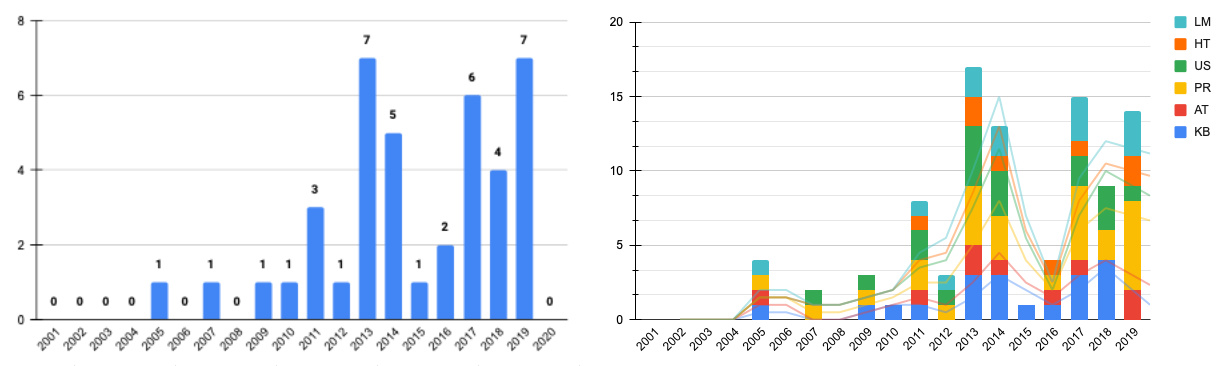
\includegraphics[width=17cm]{figures/doublechart.png}
    \caption{Trends in AR piano prototypes. \textbf{Left:} Number of articles published on AR piano within the last two decades. \textbf{Right:} Trend of contribution categories on the AR piano papers published within the last two decades. We have used moving average values to visualize the trends in these different contribution categories. }
    \label{fig:doublechart}
\end{figure*}  

This section discusses the novel contributions on AR piano prototypes based on the categories presented in Section \ref{sec: trends}. These innovations will be discussed in detail based on how they have improved in recent years, how they have been utilized in relation to the shift of focus from mobile to ubiquitous to tangible, and how they have improved learning experiences throughout the years. We reiterate again that even if there are forty (40) papers included in this review, these do not necessarily mean that there are 40 prototypes as well. In fact, some of the works illustrate incremental improvements of the same prototype throughout the years. 

\subsection{Agents and tutors}
\label{subsec: agent}

\begin{figure*}[t]
    \centering
    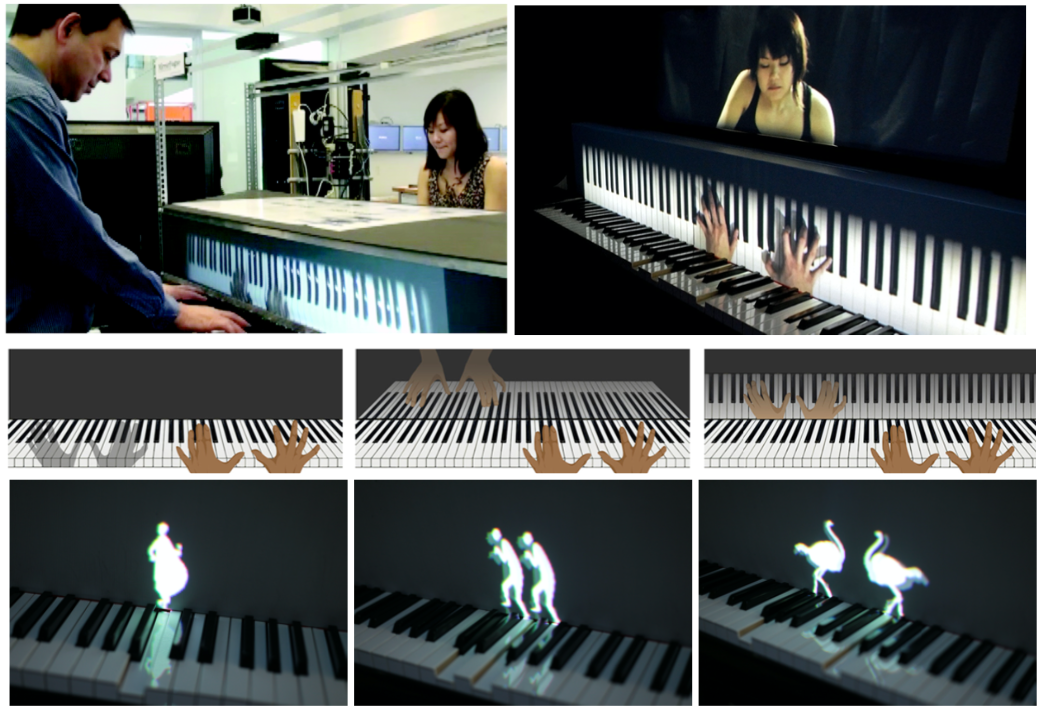
\includegraphics[width=18cm]{figures/xiao.png}
    \caption{Agents and tutors in the MirrorFugue series. \textbf{Top left:} MirrorFugue I: piano duet prototype where a tutor sits across the learner. A camera is setup on top of the hands of the tutor. This is fed and viewed into a projection that is seen by the learner positioned just above the keys of the learner. \cite{xiao2010mirrorfugue}. The goal of this prototype to communicate proper hand gestures but with collaboration as the focus. \textbf{Top right:} MirrorFugue III: this prototype \cite{xiao2013mirrorfugue} projects (they used the word \textit{"conjures"} instead of projects) a recorded pianist instead of a live pianist used in \cite{xiao2010mirrorfugue}. In this setup, it focuses on teaching the learner to press the right keys similar to that of an expert pianist as seen in the projection. \textbf{Middle:} The concept photo for the proposed interface done in the work of \cite{xiao2010mirrorfugue}. It introduces the shadow mode, the mirror mode opposite the learner and the mirror mode beside the learner. This explores the different modes on which position and posture of the visualization will fit best in teaching the right finger positioning and timing in pressing.  \textbf{Bottom:} Andante: the latest incremental improvement in the Mirrofugue series, which uses creating and dancing animations as projections instead of a the virtual pianist, as piano roll representations. The movements and steps shown by the animated figures guide the user on the tempo and the right keys to press in the piano. }
    \label{fig:xiao}
\end{figure*}

In AR piano prototypes, having an augmented reality keyboard or an interactive keyboard has been an obvious choice. These studies served as the test bed for spatial registration, rendering and optimization of graphics in mobile AR. Another addition to AR piano prototypes is the use of augmented agents and tutors. Only 9 out of 40 prototypes (22\% of the total) had virtual agents and tutors as part of their contribution. These virtual characters, at the time, were computationally-extensive but considered exciting. Some AR piano prototypes have designed augmented agents and tutors that assist the novice piano learner. The development of agents and tutors would usually have two distinct focus namely (1) designing and rendering agents to appear as human-like or as realistic as possible and (2) designing them to be as intelligent as possible. In the context of AR piano prototypes, the improved user experience has also been considered more recently. 

The MirrorFugue series \cite{xiao2010mirrorfugue, xiao2011duet, xiao2013mirrorfugue, xiao2014andante} (as seen in Fig \ref{fig:xiao}) features AR piano prototypes that attempts to address not only the two focus but also introduces a third focus for AR agents and tutors - which is to give pleasant and exciting experiences with an agent. In order to do this, they developed multiple iterations of the AR piano prototype that considers several use-cases. First, they attempted to gauge collaboration between a learner and a tutor. A regular keyboard is equipped with special cameras and projections that show to the novice, the hand movements of the more experienced user. Second, their work introduced various interfaces (shadow and reflection) and they measured which among these interfaces would best visualize the movement of the tutor in a way that is easiest for the learner. Then, they tested with various modes on how to project these reflections. One mode displayed a shadow hand beside the player. Another mode, had hands reflected from dashboard of the keyboard, giving the player a mirror's view similar to how dancers would follow a choreographer's movements. In the latest version of their prototype, they pivoted the design of their agent from a reflection to using animated agents. Their results led novices on how to play the keyboard by following the movement of these agents. As seen in Fig \ref{fig:xiao} (bottom part), augmented agents that were configured with musical notation (such as tempo, pitch, etc) dance during a performance thereby leading the user on how to play the piano. 

\begin{figure}[t]
    \centering
    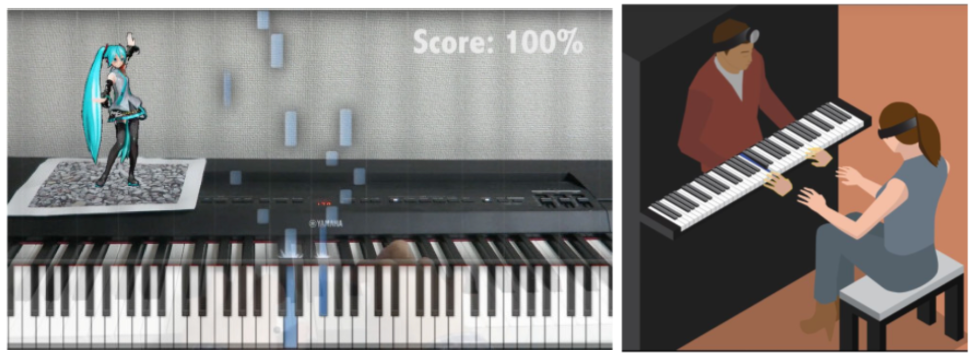
\includegraphics[width=8.5cm]{figures/goodwingerry.png}
    \caption{Featured prototypes that use agents and tutors. \textbf{Left:} The work of \cite{goodwin2013key} which was published in 2013. It was still using marker technologies to track an anime-inspired agent. It uses piano roll visualizations which were being displayed when the agent dances. It was also measuring timing and accuracy to gauge the user's performance.  \textbf{Right:} The ADEPT prototype \cite{gerry2019adept} where a user sees and embodies a piano tutor through a virtual agent. Users wear a glove which serves as guide that they can follow. }
    \label{fig:goodwingerry}
\end{figure}

The Augmented Design to Embody a Piano Teacher (ADEPT) \cite{gerry2019adept} provides a first-person audiovisual perspective of the teacher to the tutor. In other works, learners usually follow the guide or walkthrough by a tutor but in this study, they are guided by a tutor that is embodied in their point of view (POV). Learners wear a virtual glove that they see through a head-mounted display and follow the lead of a virtual tutor. This virtual tutor shows an actual person in a separate room, where their hand movements are recorded and projected as an embodiement to the vision of the learner. The work of \cite{goodwin2013key} took entertaining to the next level by using \textit{anime}\textendash inspired agents to teach piano. The agent used marker-technology for tracking and had piano roll visualization as well to guide the user. 

\subsection{Piano roll and other visualisations}
\label{subsec: viz}

\begin{figure}[h]
    \centering
    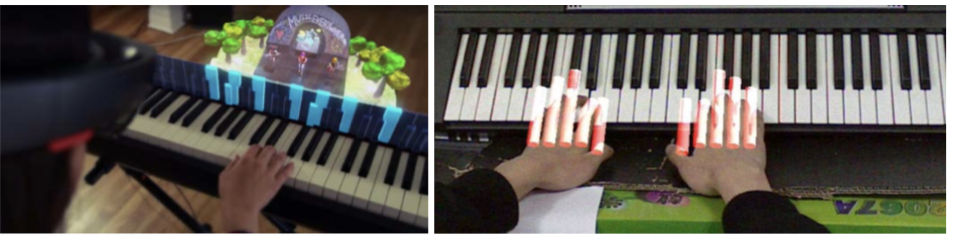
\includegraphics[width=8.5cm]{figures/dashuang.png}
    \caption{Stationary piano roll visualizations in head-mounted displays. \textbf{Left:} The AR piano prototype described in the work of \citet{das2017music}. In this mixed reality setup, users wear a headmounted display where they see piano roll visualizations by the edge of the keyboard thereby guiding the users on what specific keys to press. An agent performer is also seen to entertain the piano player, moving depending on the rhythm provided. \textbf{Right:} The AR piano prototype described in the work of \citet{huang2011piano}. A user wears a head-mounted display while operating a real piano. The mobile device in the head-mounted display sees the piano and renders graphics on top of the keys, guiding the user on which key to press. The visualizations on both of these studies appear stationary.  }
    \label{fig:dashuang}
\end{figure}

The most cited difficulty in learning how to play the piano is the learning curve introduced by the music sheet notation. This is why a popular approach (26 out of 40 \textendash  which is 67\% of these prototypes)for this problem is to use interactive piano roll visualizations. Piano roll visualizations in AR are music visualizations that novice players can use. They serve as an easier representation to read complex music sheet notation, enabling novice users to quickly learn the piano \cite{walder2016modelling}. In this approach, the learning curve is reduced as novices need not to learn (yet) complex music notation and can focus on proper finger positioning, placement and accuracy. These visualizations usually come in polyphonic form to represent multiple melodies that take place in the same concurrent time segment \cite{ciuha2010visualization}.  Piano rolls have been used as well such for the guitar \cite{biamonte2010musical}, drum \cite{rossignol2015alternate} and many others. It is important to note that piano roll visualizations do not necessarily mean they are visualizations for piano. But rather, they represent a group of visualizations that move and unveil sound information as the visualizations are reveled, similar to the traditional piano roll music box. In general, piano roll visualizations refer to a group of visualizations that behave similarly with movie credits, rhythm games and many others. 


Piano roll visualizations are designed to guide users on which key to press at the right time. This gives the spatiotemporal component (\textit{spatio} - position in multidimensional space, and \textit{temporal} - movement with consideration of time as the major element) depending on the platform and environment where they are implemented. The graphics are usually overlaid near or on top of the piano keys moving (either be downwards or sideways depending on the target) towards the button that the user should press. 

These visualizations used for AR prototypes have appeared in different forms. AR piano prototypes that are mobile-based or that may need a head-mounted display would render their piano roll visualizations to show as if they were on top of a real piano. On most cases, these visualizations appear on top of the piano keys seen through the camera of the mobile device (see Fig \ref{fig:dashuang}). Some of them are stationary and do not move, serving only as visual stimuli waiting for the user to input and press the key below them. Some visualizations are non-stationary, actively moving towards the keys to press, based on a given song's tempo (see Fig \ref{fig:caitrujano} Left ). Some of them have been found on AR prototypes where they display piano roll visualizations outside of the mobile device or head-mounted display. These AR piano prototypes have been designed to display visualizations in wider spaces through a 3D projector or specialized cameras like the Kinect. These moving visualizations denote extra meaning, sometimes sending additional feedback to the users. They may appear in a given color (usually blue or any neutral color) to denote that they should be pressed next (or soon). Then they appear in a different color to denote the success of the pressing (green for good timing, yellow for somewhat delayed timing and red for missed or wrong key pressed) (see Fig \ref{fig:caitrujano} Right and Fig \ref{fig:projectors}). 

\begin{figure}[t]
    \centering
    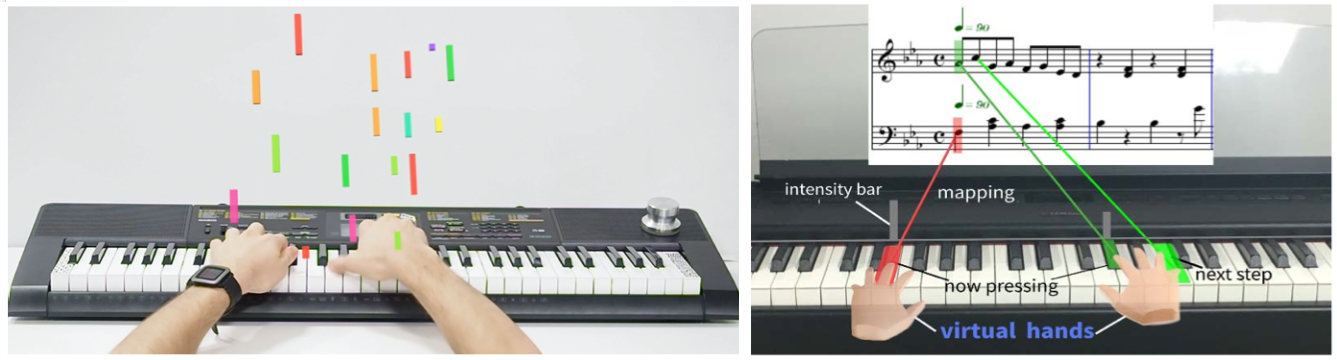
\includegraphics[width=8.5cm]{figures/caitrujano.png}
    \caption{Moving piano roll visualizations in head-mounted displays. \textbf{Left}: The piano roll visualizations in the prototype by  \cite{trujano2018arpiano} uses a head-mounted display and uses a minimalist interface. Key visualizations appear in random colors and seem to come out of nowhere. As the graphics draw closer to their respective keys, they slowly fade. No feedback exists to show whether the keys pressed are correct or not.  \textbf{Right}: Preview of the architecture of the prototype described in \cite{cai2019design}. The prototype uses \textit{"intensity bars"} as piano roll visualizations that appear in two colors: red (now pressing) and green (next to press). These intensity bars are mapped directly with their equivalent notes as seen in the music sheet. Virtual hands are displayed as well in helping the user position their hands. }
    \label{fig:caitrujano}
\end{figure}

There are also specific types of piano roll visualizations that are non-stationary. These visualizations appear to move within a specific time frame giving the user the notion of temporality (see Fig \ref{fig:caitrujano}). As these visualizations move, they teach two things to the user: (1) knowing the right key to press at the right time and (2) mapping the complex music notation and their equivalent key press. Some of these piano roll visualizations have also been introduced in a gamified mode \cite{Weing:2013:PEI:2494091.2494113} which researchers believe allowed learners to learn faster or easier. More on these learning modes will be discussed in subsection \ref{subsec: learn}. 

%It is interesting to note that piano roll visualizations used in AR piano prototypes have been consistently appearing in the past 15 years. Whether they are displayed through a mobile device, or a head-mounted display or projected through a large interctive space, the quality and speed also improves. 



\subsection{Evaluation techniques introduced through user studies}
\label{subsec: eval}

Of the 40 papers included in this review, only 18 (45\% as seen in Table \ref{tab:overview}) have performed user studies on the system  as part of their contribution. These user studies evaluated certain factors such as ease of use, satisfaction, immersion, motivation and performance among many others. We believe that through the development of AR piano prototypes, techniques and methods on evaluating these factors have changed and improved as well. Following the data gathering techniques described in subsection \ref{subsec: gathering}, we reviewed these papers and analyzed how they did their user studies. We looked at their sample size, the type of their participants, the type of treatment, the metrics or constructs they measured and the tools/instruments they used to measure these metrics. In our review, we observed a shift of focus in treatment and metrics in the same way the shift in focus for visualizations and agents/tutors have taken place. 

What separates HCI research from other disciplines is it properly gauge the impact of the prototypes, systems into their human users. Specific human factors and affordances are usually discovered as these user studies are done. We begin looking at these evaluation techniques introduced with the participants involved and their respective size. The number of participants involved in these studies ranged from 1 to 74, with a median sample size of 8.5 (see Table \ref{tab: us-all}). These involved a combination of expert and novice users, people with or without background in using AR apps and tools. There was even one study who involved patients with disabilities as part of their respondents \cite{correa2009computer}. These studies considered various study designs from between-subject, within-subject, with or without control groups and many others. Since there are other contribution categories introduced by these papers, they have different focus in terms of treatment (see Table \ref{tab: us-all}). These were also depending on the year the studies were published from (either between 2005-2010, 2011-2015 or 2016-2020). Earlier studies tend to measure usability in consideration accuracy of spatial registration (such as marker detection). Newer studies focused on measuring activities where users are more free (or have more flexibility) to play around with the tool. These studies have their users do task-oriented use cases (such as playing major or minor chords \cite{nugraha2014pemanfaatan, xiao2010mirrorfugue}, play a specific song or piano piece \cite{chow2013music, sandnes2019enhanced,pan2018pilot} or simply practice the piano on their own for a specific amount of time \cite{weing2013piano, raymaekers2014game}). In some studies, adding familiar and entertaining elements have allowed experiments that focused on gamification, and the ability of the users to complete quests as an alternative approach to measuring performance and learning. 

% Please add the following required packages to your document preamble:
% \usepackage{graphicx}
\begin{table*}[t]
\caption{List of studies with user evaluation (labelled as \textbf{US} as seen from Table \ref{tab:overview}). This table provides an overview of their treatments, metrics, constructs and tools used.}
\label{tab: us-all}
\resizebox{\textwidth}{!}{%
\small\begin{tabular}{lcllllll} \hline \hline
\textbf{Ref.}                           & \textbf{Size} (\textit{n})    & \textbf{Treatment}    & \textbf{Metrics or constructs}    & \textbf{Tools} & \textbf{Notes }\\ \hline
%P1 \cite{huang2011piano}              & 2011 &        & a                         & a                             & a                    \\
\cite{nugraha2014pemanfaatan}        & 8        & md, pc    & At, Op, Us        & SMQ                   & \\
\cite{chow2013music}                 & 7        & pl        & Sa, Us        & OEQ                   & \\
\cite{weing2013piano}                & 5        & ex, pr    & CL, FI, No, Sa    & SMQ                   & \\
\cite{kerdvibulvech2017innovative}  & 1         & pl        & Sc, TI            & TTM                   & \\
\cite{schmalstieg2007experiences}   & 6         & pl, qu    & Sa, TI            & PSP, SSI, TTM         & \\
\cite{correa2009computer}           & 1         & ex, qu    & Op, Us*           & REC, TTM              & \textit{*patient motor effects} \\
\cite{takegawa2012piano}            & 9         & pl, pr    & FI, No, Sc, TI    & PSP, SSI, TTM         &   \\
\cite{xiao2010mirrorfugue}          & 5         & pc, pl*   & Im, Op            & PSP, REC, SSI, TTM    & \textit{*improvise a piece}\\
\cite{xiao2013mirrorfugue}          & 15        & ob        & Im, Op, Us        & SMQ, SSI              &  \\
\cite{li2018application}            & 17        & ex, ob    & Mo, Op            & QUE*                  & \textit{*instrument from }\cite{zhang2000relationship}    \\
\cite{leonard2013virtual}           & 20        & ex, pr    & Op, Sa, Sk        & OEQ, TTM              &    \\
\cite{raymaekers2014game}           & \textendash* & ex, pl, pr & At, Sa, Us    & OEQ, REC              & \textit{*open demo UT} \\
\cite{rogers2014piano}              & 74*       & pc, pl, pr & At, CL, Sa, Sk, Us, TI & QUE\dagger      & *$n_{1}$=56, \begin{math}n_{2}\end{math}=18, $\dagger$\cite{ekstrom1976manual, klepsch2012subjective, hassenzahl2003attrakdiff, wrigley2013ecological}\\
\cite{sun2018mr}                    & 20        & ex, pc, pl & Sc, Sk, Us, TI   & PSP, TTM              &   \\
\cite{molloy2019mixed}              & 23        & pl        & At, Im, Mo, Us    & OEQ, QUE*, SSI        & *SUS \cite{lewis2009factor}\\
\cite{pan2018pilot}                 & 13        & pl, pr    & Sc, Sk            & OEQ, PSP, SMQ, SSI    &  \\
\cite{kim2014ar}                    & \textendash* & ex, md    & FI, Op         & REC                   & \textit{*n not reported}  \\
\cite{xiao2011duet}                 & 3         & ex, ob    & Im, Us            & SSI                   &   \\ \hline 
                                   & \textit{med.}=8.5 & \textit{\={x}}=14.19   &                   &                       & \\ \hline \hline 
\end{tabular}%
}
\caption*{\textbf{Treatment Legend}: \textbf{ex}= free usage and exploration modes; \textbf{md}= marker detection; \textbf{ob}= observation of prototype usage; \textbf{pc}= play piano chords on the piano;  \textbf{pl}= play a piece in the piano; \textbf{pr}= practice the piano; \textbf{qu}= complete quest in a game or gamified interface.  \textbf{Metrics Legend}:   \textbf{At}= attractiveness; \textbf{CL}= cognitive load; \textbf{FI}= accuracy of finger information; \textbf{Im}= level and quality of immersiveness; \textbf{Mo}= level of user motivation; \textbf{No}= accuracy of notation; \textbf{Op}= functional check of the different features of the prototype; \textbf{Sa}= satisfaction rating of the prototype; \textbf{Sk}= improvement in skill; \textbf{Us}= ease of use and usability; \textbf{TI}= time interval and usage of the system; \textbf{Sc}= scoring (for gamified prototypes). \textbf{Tools Legend}: \textbf{OEQ}= open ended questionnaires; \textbf{QUE}= used a peer-reviewed questionnaire/instrument; \textbf{PSP}= player scoring plug-ins; \textbf{REC}= observations from recordings; \textbf{SMQ}= self made questionnaire; \textbf{SSI}= semi structured interviews; \textbf{TTM}= time tracking mechanisms. }
\end{table*}

The introduction of task-oriented use-cases in evaluating usability in these AR piano prototypes led to the use of newer metrics and/or constructs that properly-describe them. Metrics that used to be difficult to measure are now defined in these newer studies thanks to recent innovations as well. Earlier AR prototypes focused on measuring attractiveness and function. Since AR technologies allow a person to be immersed between virtual and actual reality \cite{milgram1995augmented}, metrics that define immersion (how a person is immersed in an AR artifact) have been used as well. As users get immersed, this leads to significant impacts in cognitive load and their state of being overwhelmed. Cognitive load, and other affect measures such as user motivation give additional insight on the usability of these AR prototypes as well. These constructs allowed AR piano prototype researchers to finally look at the core important factor which is piano learning without having to think of specific implementation issues (such as spatial registration, object tracking, etc). In order to fully understand and accurately-assess piano learning, additional metrics have also been considered such as time interval, key-press accuracy, mastery of music notation, scoring based on hit-miss accuracy and other skill improvement measures. There were other specific metrics or constructs observed in these studies that are considered unique or not well-investigated such as the impact of AR on motor effects of patients with cerebral palsy, how the interface supports team-play and collaboration among multiple users and many others. 

Along with the development of metrics or that assess piano skill learning, are the introduction of tools and instruments that support these constructs. In these user studies, observations, interviews (both pre and post) allowed AR piano prototype developers to understand their users and the insights they discover deeper. Some studies consider a mixed-method design where they employ plug-ins and programs that measure specific indicators (quantitative - such as tracking of key-press, recording of time intervals between practices, assigning points in gamified modes; qualitative - such as think out aloud protocol, facial expressions observed by coders and annotators, etc). Studies that measured cognitive load have used advanced sensors such as galvanic skin response (GSR) and electrocardiogram (ECG). It is interesting to note that a great number of the studies reviewed in this paper have used their own self-made questionnaires (see label \textbf{SMQ} in Table \ref{tab: us-all}). The use of semi-structured interviews along with these self made questionnaires have been a popular choice for their study design. Only a few studies have used peer-reviewed and established questionnaires and instruments (such as Attrakdiff \cite{hassenzahl2003attrakdiff} and SUS \cite{lewis2009factor})  in their study design. Some articles reviewed did user studies in informal settings where participant criteria and sampling were not clearly-defined or were not restricted to a specific demographic type. 

Other evaluation methods and tools demonstrated their specific advantages and disadvantages depending on how the studies were done. For example, semi-structured interviews and observations were more helpful in understanding usability factors in using AR piano prototypes. Expert reviews played a crucial role in measuring learning and skill improvement. Having control groups in between user studies of these AR piano prototypes allowed researchers to understand if there are actual improvements introduced by these prototypes (measured by ANOVA, significant difference and other statistical tools) as compared to the traditional setup of using the piano. 

%done by studies on AR piano teaching systems (hypothesis based on cognition, realistic annotations etc)

\subsection{Hand tracking}
\label{subsec: ht}
Im still studying HT. prolly last that I will write

\begin{figure}[t]
    \centering
    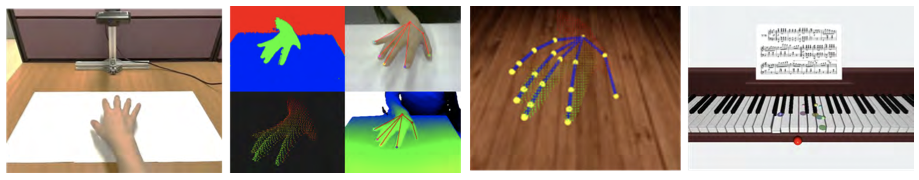
\includegraphics[width=8.5cm]{figures/lianghandtrack.png}
    \caption{Different forms of hand tracking for the piano done in the work of \cite{liang2016barehanded}. It considers lighting and how a hand is placed on top of a white background (\textbf{first}), segments the hand based on image processing techniques (\textbf{second}), identifies joints and action points of the fingers in the (\textbf{third}) and its positioning in an augmented piano (\textbf{fourth}). }
    \label{fig:lianghandtrack}
\end{figure}

Text here. 

\subsection{Learning modes}
\label{subsec: learn}

\begin{figure*}[t]
    \centering
    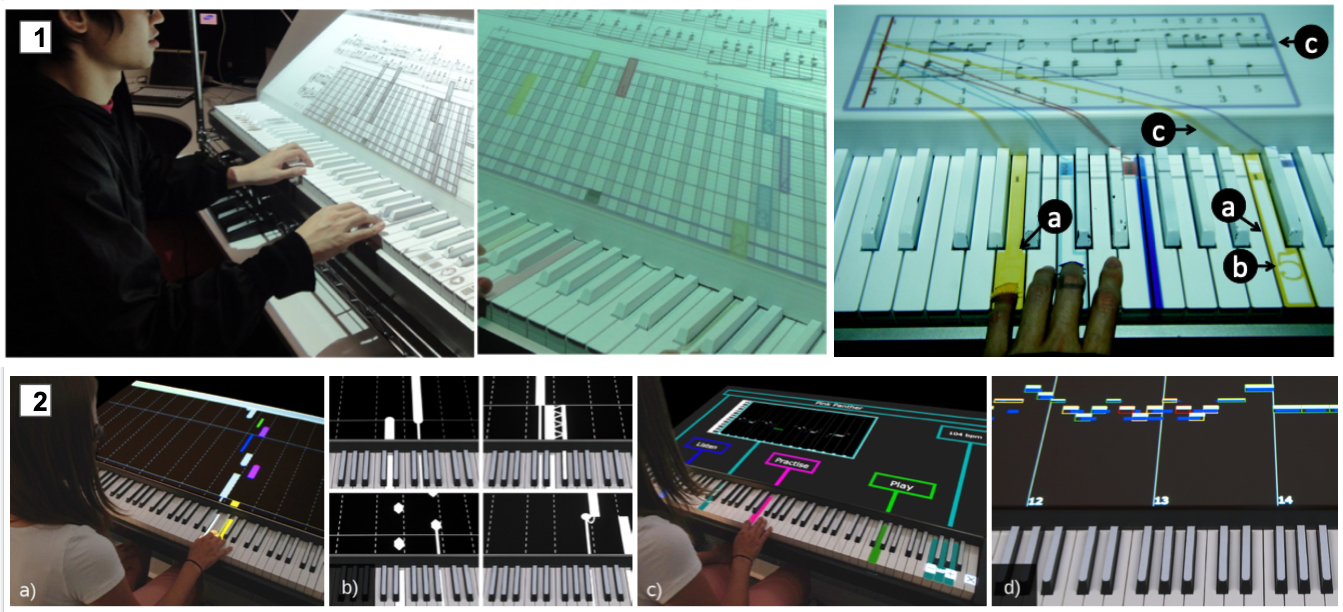
\includegraphics[width=18cm]{figures/projectors.png}
    \caption{Projector-based visualizations and their learning modes.  \textbf{\#1}: The prototype by \cite{takegawa2012piano}. It utilizes a projector that displays the piano roll visualizations on top of an actual piano. The black keys in the piano have been recoloured to white. Specific colored visualizations appear on top of each keys guiding the user on what and when to press. A music notation sheet which is drawn with colored lines are mapped to the piano roll notations that overlay the piano keys. In their approach, the music sheet is transformed into lines, which point to piano roll visualizations that are overlaid on top of the keys that the users can press. \textbf{\#2}: The prototype in \cite{rogers2014piano} which uses a similar projection technique with that of Takegawa et al. However, their prototype introduces learning modes which change how the piano roll visualizations are displayed. Depending on the mode, the piano roll can move downwards similar to that of rhythm games, or like building blocks that are read from left to right. }
    \label{fig:projectors}
\end{figure*}

One main concern as to why we build AR piano prototypes is because we want to help piano learners in the learning process. Developers have created AR piano prototypes in a way that is considers the context of learning, skill improvement for piano novices. This was done by introducing various learning modes which began to emerge in the latter era. Of the 18 articles (as described in subsection \ref{subsec: eval}), only 7 (17\% of all the articles covered, 38\% of US-studies) incorporated learning modes as part of their contribution. Another 5 articles (who did not have a user study as part of the contribution) introduced learning modes as well as part of their prototype - but these were not evaluated in a user study. A Practice mode has been a common part of these learning modes. A self-reflection learning mode has also been introduced by a few studies \cite{gerry2019adept, xu20195, xiao2013mirrorfugue}. In this mode, users of the AR piano prototypes can watch and view their own performance - either in real time or after an experiment treatment. We believe that this feature is draws inspiration from the theory of \citet{zimmerman2009self} on how self-reflection promotes self-regulated learning as seen on some various learning experiments \cite{deja2016discovering,lyons2011monitoring}. Since AR piano prototypes were developed as an alternative learning environment for piano learning especially when a tutor is absent or when learning can take place on its own, a learning mode such as self-reflection definitely supports this process. 

Aside from self-regulation and self-reflection theory, social learning theory emphasizes four distinct steps in learning namely attention, retention, reproduction and motivation \cite{bandura1977social}. In \textit{attention}, a piano learner observes a process. During \textit{retention}, the piano learner performs activities where they try to remember what they have observed (from the previous step). The \textit{reproduction} then follows this where they perform activities that they have observed. This learning process becomes sustainable that it leads to medium to long-term improvement through the \textit{motivation} step. Here, reinforcement (could be positive or negative) ensures that the novice can continuously practice and learn the piano. The prototype described in the work of \citet{weing2013piano} and \citet{rogers2014piano} supports social learning theory through their design of their learning modes. 

A \textit{listen (attention)} mode allows novices to observe and listen in a song that is visualized in their AR piano prototype. They considered this mode based on inputs with experts involved in their study. The \textit{practice (retention)} provides novice players a different form of piano roll visualization (as seen in Fig \ref{fig:projectors}). They believe that retention is maintained by showing users of their AR piano prototype the correct way of playing the keys and allowing them to perform them without haste. In this learning mode, feedback in the form of visualizations, brightly highlights the correct keys and the wrongly-pressed keys. Lastly, in their \textit{play (reproduction and motivation)} mode, users of the AR piano prototype can receive additional feedback on their performance. They can play a specific song or piano piece \textit{(reproduction)} following a form of piano roll visualization different from practice mode. As users play in this mode, they receive live feedback on their key press. Similar to rhythm games, they also get to see a summary of their performance through a progress bar. With the help of player scoring plug-ins (PSP) and time-tracking mechanims (TTM) (as seen in Table \ref{tab: us-all}), an additional layer of information is shown about their performance. Not only do they see correct or mis-pressed keys, expected notes (missed keys), incorrect duration are also displayed. By self-reflection and seeing an overview of their performance, piano learners are expected to reflect on their progress both at an abstract and low level of detail, which in turn provides \textit{motivation}.

\begin{figure}[t]
    \centering
    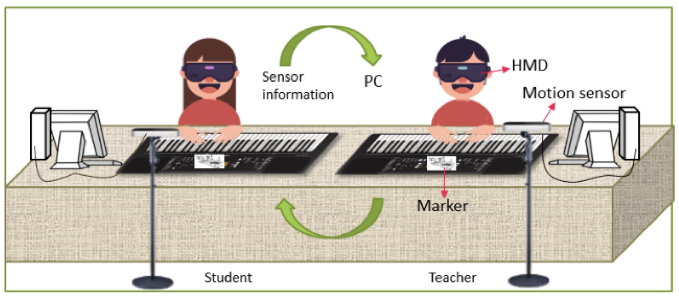
\includegraphics[width=8.5cm]{figures/caigroup.png}
    \caption{Multi-user collaboration. In the work described in \cite{cai2019designb} a setup has been designed where at least two users equipped with head-mounted displays can co-perform a musical piece in the AR piano prototype. They do this by pressing keys following the piano roll visualizations that have have to be pressed and completed by both users. It can be used on two modes, a competitive mode and a collaborative mode where in the former they aim to get a score higher than the other and in the latter, they try to cooperate and work together on a single piano piece.}
    \label{fig:caigroup}
\end{figure}

Other modes of interaction have also been introduced to aid learning and other piano-related activities. Learning with a partner \cite{xiao2011duet}, performing with a group \cite{gerry2019adept} and learning with a group \cite{cai2019design}. Other AR piano prototypes also included a competitive mode \cite{cai2019designb} to encourage learners to perform better during piano practice. 

\section{Discussion and Future Directions}
\label{sec: discuss}
gaps in modelling? position near your thesis

text here



%%
%% The next two lines define the bibliography style to be used, and
%% the bibliography file.
\bibliographystyle{ACM-Reference-Format}
\balance
\bibliography{sample-base}

%%
%\nocite{*}
%% If your work has an appendix, this is the place to put it.
%\appendix
\end{document}
\endinput
%%
%% End of file `sample-manuscript.tex'.
